A concurrent program is any program consisting of multiple units of execution
that work together towards some common goal.  Each unit of execution has its
own thread of control: it has its own local state.  The different units might
also have some shared state, such as shared variables.  

The units of execution might all execute on the same processor, sharing
processor time.  Or they might operate on several close-coupled processors,
within a single computer.  Or they might be distributed across a network.

We will see various patterns for how the units work together.  For example,
they might be performing different operations, as part of a pipeline; or they
might be performing the same operation, but on different parts of the data.
%
The key concern in each case is coordinating the different units tasks, to ensure
correct sequencing of interactions or communications between them.

%%%%%%\heading{Processes and threads}

Units of execution can be implemented as either processes or threads.
%
A~\emph{thread} is a single sequentially executing program.  At each point, it
is at a particular place in the program, and has its own \emph{thread-local}
variables and control stack.  However, different threads may share memory, and
so communicate with one another via shared variables.  This provides for a low
communication overhead.  Threads are normally fairly lightweight, so context
switching (where a processor switches from executing one thread to another)
can be cheap.

A \emph{process} consists of one or more threads sharing an address space
(i.e.~area of memory).  However, different processes have separate address
spaces.  This protects processes from each other.  But it means that processes
cannot communicate via shared variables.  Instead they communicate with each
other either using operating-system calls, or by communicating over a network,
which means that they have relatively high communication overheads.

In this book we will write programs that use threads sharing a single address
space.  However, some of our programs use message passing (only), so the
threads could be replaced by processes in distinct address spaces, or even on
different computers.

The word \emph{concurrent} refers to two or more threads or processes that
overlap in time.  However, they might not ever be running at precisely the
same instance.  Instead, a processor could be switching between them,
timesharing.

By contrast, the word \emph{parallel} means that the threads or processes are
running at the same time, on different hardware.  We will not distinguish much
between concurrency and parallelism in this book.  All of our programs could
run on a single processor, time sharing.  However, we really expect them to
run in parallel, on different processors, so as to give faster performance.

%%%%%%%%%%%%%%%%%%%%%%%%%%%%%%%%%%%%%%%%%%%%%%%%%%%%%%%%%%%%

\section{Reasons for concurrency}

Why should we write concurrent programs?

The most obvious reason for using concurrency is that running a program on
multiple processors in parallel will often make the program faster.  Examples
include scientific computations (e.g.~modelling the climate, the evolution of
a galaxy, or the effects of new drugs), graphics and image processing, and
combinatorial or optimisation problems (e.g.~scheduling problems, or
game-playing algorithms).  \framebox{Improve -- ``AI''}

Often these programs employ \emph{data parallelism}: each thread or process
works on part of the data, with all working in the same way; perhaps there
might also be one or more coordinating threads.  Very large computations may
well be distributed over multiple computers, communicating over a network.

As we will see, using concurrency does not necessarily make a program faster.
There is a danger that the communication and coordination costs outweigh the
benefits of using extra threads.  Some judgement and experimentation is
necessary to achieve good performance. 

%%%%% Reasons for concurrency: (2) multi-task systems

Another reason to use concurrency concerns multi-task systems.  Many systems
are responsible for a collection of independent or semi-independent tasks,
each with its own data, although with some interaction between tasks.  Such
systems are easier to program using a single thread or process per task,
rather than having a single monolithic thread that is responsible for all the
tasks.

Examples include real-time controllers for factories, power plants,
spacecraft, etc.  Here, the different components can mostly operate
independently, with just occasional interactions.  Another example is an
operating system, where separate components, such as scheduling and allocation
of memory or disk space, can sensibly be performed by different processes.
Likewise, in a simulation, different threads may simulate different components
of the simulation.  And in a multi-character game, different threads may
control different characters.

Concurrency is often used within graphical user interfaces (GUIs).  For
example, in Swing, a special thread, the \emph{event dispatch thread}, is
responsible for handling all GUI events.  However, if this thread were
responsible for any long-running computation, it would make the GUI
unresponsive.  A better approach is for the event dispatch thread to arrange
for some other thread to perform the computation. 

%% For example, consider a controller for a light, that turns the light on and
%% off periodically.  Using appropriate library code:
%% %
%% \begin{scala}
%% def controller(light: Light, tOn: Int, tOff: Int) = {
%%   private var tBase = getCurrentTime
%%   while(true){
%%     light.on; sleepUntil(tBase+tOn)
%%     light.off; sleepUntil(tBase+tOn+tOff); tBase = tBase + tOn + tOff
%%   }
%% }
%% \end{scala}

%% Now suppose you need to control 1000 lights.  
%% %
%% \begin{itemize}
%% \item
%% How would you do this with a sequential program?

%% \item
%% With a concurrent program it is easy: create one thread or process for each
%% light, and run them concurrently.
%% \end{itemize}

In such multi-threaded multi-task systems, multiple threads or processes run
concurrently on the same processors, often with more threads or processes than
processors.  The threads or processes take turns to use the processors, under
the control of the operating system.

%%%%% \heading{Reasons for concurrency: (3) distributed computing}

The third main reason for using concurrency is where an application makes use
of services provided by computers that are physically distributed.  Such
applications are necessarily concurrent, involving interactions between
processes running on different computers.

Examples include:
\begin{itemize}
\item The World Wide Web, where exchanges take place between web
clients (e.g.~a web browser) and web servers; 

\item Distributed file systems, where exchanges take place between users'
  computers and file servers;

\item Database systems, where client computers interact with a database
  server;

\item Wireless sensor networks, where spatially distributed sensors monitor
  the environment (e.g.~for pollution, temperature, or sound), and return
  results to a central location;

\item Unmanned autonomous vehicles (drones), that communicate with a central
  location to receive commands and send back data (e.g.~video);

\item Fault-tolerant systems, that use redundant hardware, where components
  communicate together to identify and overcome faults. 
\end{itemize}

These applications often use a client-server architecture, where a client
makes a request to a server, which produces a suitable response.  We will
study the client-server paradigm in Chapter~\ref{chap:clientServer}, mainly in
the concept of non-distributed systems, but many of the same techniques apply
in both settings.

The components might themselves be multi-threaded.  For example, most web
servers are multi-threaded, with a separate thread being created for each
request.  This provides the obvious advantage of providing greater throughput.
It also simplifies the structure of the server: it is easier to implement
multiple threads, each of which has to deal with a single connection, than a
single thread handling multiple connections.  Further, an organisation might
using multiple, distributed servers, with a form of load balancing, to provide
greater throughput and fault tolerance.

%%%%%%%%%%%%%%%%%%%%%%%%%%%%%%%%%%%%%%%%%%%%%%%%%%%%%%%%%%%%

\section{Concurrent architectures}

We now briefly describe a few different concurrent architectures, to provide
background for the rest of the book.

%%%%% 

\subsection{Uni-processor multi-threaded systems}

Until early this century, most personal computers had a single processor.
However, they could run multiple processes, belonging to the user or the
operating system.
%
In such systems, the operating system is responsible for sharing the processor
between threads.  The operating system selects a suitable thread and executes
it until either the thread suspends itself, e.g.~waiting for input or output
to complete, or the thread has used up its time allocation, at which point it
is interrupted.  A new thread can then be scheduled.

%%%%% \heading{Thread states}

%\includegraphics[width=12cm]{Pics/threadstates.eps}
\begin{figure}
\begin{center}
%\tikzstyle{every node}=[minimum height = 9mm]
\tikzstyle{place}=[draw, rounded corners, minimum height = 8mm]
%\def\nodeHeight{minimum height = 9mm}
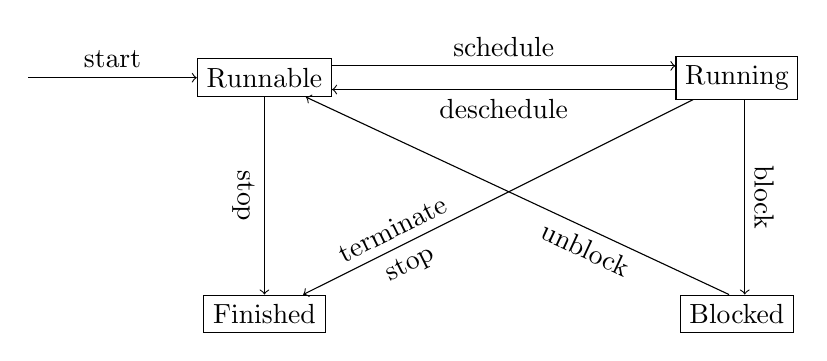
\begin{tikzpicture}
\draw(0,0) node[place](runnable){Runnable};
\draw[<-] (runnable) -- node[above]{start} (-3,0);
%
\draw(6,0) node[place](running){Running};
\draw[->] ([yshift = 1.5mm] runnable.east) -- node[above]{schedule} 
  ([yshift = 1.5mm] running.west);
\draw[->] ([yshift = -1.5mm] running.west) -- node[below]{deschedule} 
  ([yshift = -1.5mm] runnable.east);
%
% \draw (3,3) node[draw, rounded corners](waiting){Waiting};
% \draw[->] (running) -- node[above, sloped]{\scalashape wait} (waiting);
% \draw[->] ([xshift = -1mm] waiting.south) -- node[above, sloped]
%   {\scalashape notify} ([xshift = -1mm] runnable.north);
% \draw[->] ([xshift = 1mm] waiting.south) -- node[below, sloped]
%   {spurious wake-up} ([xshift = 1mm] runnable.north);
%
\draw (0, -3) node[place](finished){Finished};
\draw[->] (runnable) -- node[below, sloped]{stop} (finished);
\draw[->] (running) -- node[above, sloped, near end]{terminate} 
  node[below, sloped, near end]{stop} (finished);
%
\draw(6, -3) node[place](blocked){Blocked};
\draw[->] ([xshift = 1mm] running.south) -- 
  node[above, sloped]{block} ([xshift = 1mm] blocked.north);
\draw[->] ([xshift = -1mm] blocked.north) -- 
  node[below, sloped, pos = 0.32]{unblock} 
  ([xshift = -1mm] runnable);
%
% \draw(7, 3) node[draw, rounded corners](IOblocked){IO Blocked};
% \draw[->] ([xshift = -1mm] running.north) -- 
%   node[above, sloped]{block for IO} ([xshift = -1mm] IOblocked.south);
% \draw[->] ([xshift = 1mm] IOblocked.south) -- node[below, sloped]{complete IO} 
%   ([xshift = 1mm] running.north);
\end{tikzpicture}
\end{center}
\caption{Thread states.}
\label{fig:thread-states}
\end{figure}

%%%%%

Figure~\ref{fig:thread-states} illustrates different states a thread can be
in.  When a thread is started, it is runnable.  However, it has to wait to be
scheduled before it can actually run, i.e., be executed on a processor.  When
it is running, it can be descheduled.  Alternatively, it might block, for
example, to wait for input or output; when it is unblocked, it becomes
runnable again.  Alternatively, it might either terminate or be stopped.  (We
will consider an extension of this diagram later.)

%%%%% 

\subsection{Shared-memory multiprocessors}

Figure~\ref{fig:multi-arch} illustrates a simple shared-memory multiprocessor
architecture.  Several processors (typically CPUs) share one or more memories
(typically RAM).  They are connected by an interconnection network, for
example, a memory bus.  Thus, the different processors can read from and write
to the same addresses in the memories.  The hardware itself can only deal with
a limited number of simultaneous operations, so this can lead to contention,
both for the memory and the memory bus.  The shared memory might be organised
hierarchically, particularly in a system with many processors.

%%%%%

\begin{figure}
\tikzstyle{place}=[draw, minimum height = 8mm]
\begin{center}
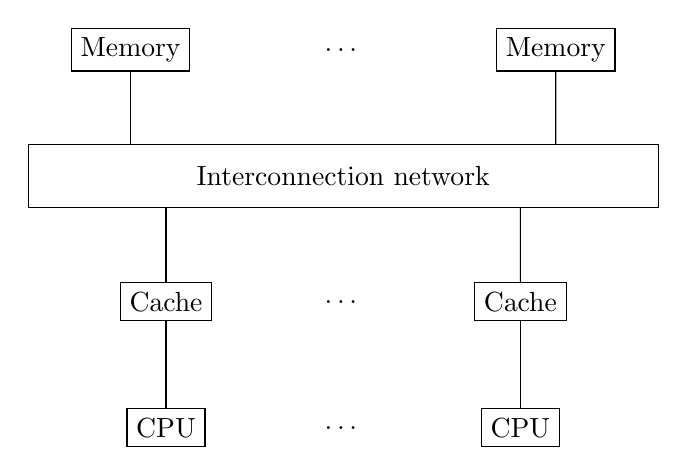
\begin{tikzpicture}[xscale = 0.9,yscale = 0.8]
\draw(0,0) node[place](mem1){Memory};
\draw (3,0) node{\ldots};
\draw(6,0) node[place](memn){Memory};
%
\draw(3,-2) node[draw, minimum height = 8mm, minimum width = 8cm]
  {Interconnection network};
\draw (mem1) -- ++ (0,-1.50); \draw (memn) -- ++ (0,-1.50); % Hack
%
\draw (0.5, -4) node[place](cache1){Cache};
\draw (3,-4) node{\ldots};
\draw (5.5, -4) node[place](cachen){Cache};
\draw (cache1) -- ++ (0,1.50); \draw (cachen) -- ++ (0,1.50);
%
\draw (0.5,-6) node[place](cpu1){CPU};
\draw (3,-6) node{\ldots};
\draw (5.5, -6) node[place](cpun){CPU};
\draw (cpu1) -- (cache1); \draw (cpun) -- (cachen);
\end{tikzpicture}
\end{center}
\caption{A shared-memory multiprocessor architecture.}
\label{fig:multi-arch}
\end{figure}

Accessing shared RAM is moderately slow (typically 10--100\,ns per operation).
Therefore modern processors have much faster cache memory, located on the same
chip as the processor.  Values read from the main memory are copied into the
cache.  A subsequent read of the same address will read that value from the
cache, which is much faster (typically around 1\,ns).

If the processor needs the contents of an address that is not in the cache,
this is known as a \emph{cache miss}.  At this point, a block of memory,
typically 64~bytes, known as a \emph{cache line}, is read into the cache in
one go.  This means that if the processor subsequently reads a nearby memory
location, for example in the same object or array, it is likely to already be
in the cache, improving performance.
  
If a processor writes to an address, that write initially happens just in the
cache, and is later copied back to the main shared memory.

Different processors may read and write the same location.  This can be
problematic if the different caches are not consistent.  If one processor
writes to an address, and then another processor reads that address, it is
possible that the update has not propagated from the first processor's cache,
or that the second processor reads a stale value from its cache.  

The specification of most programming languages include a \emph{memory model}
that defines the degree of consistency that is guaranteed.  In Scala (and
Java) this is the \emph{Java Memory Model}.  We will describe later
circumstances under which a read at one processor can be guaranteed to see the
results of an earlier write at a different processor.

%% It is therefore important to keep different caches consistent.  See the
%% Architecture course for details.

%%%%% \heading{Multi-core processors}

Nowadays, most processors have multiple cores on the same chip.
Figure~\ref{fig:multicore} gives an example of an eight-core chip: each CPU
has its own level~1 data cache (L1d; e.g.~16K), shares a level~1 instruction
cache (L1i; e.g.~64K) and a level~2 cache (L2; e.g.~2048K) with another CPU,
and shares a level~3 cache (L3; e.g.~8192K) with all the CPUs on the chip.

%%%%%

\begin{figure}
\begin{center}
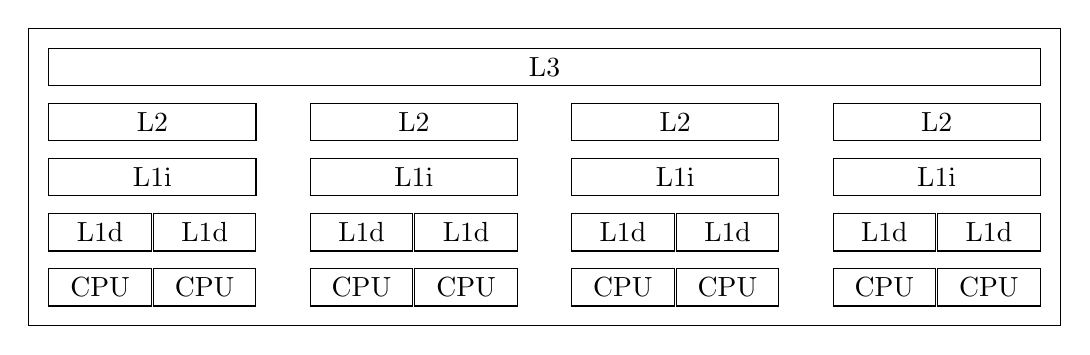
\begin{tikzpicture}[xscale = 1.66, yscale = 0.7]
%% \foreach \x in {0,1,...,7}{
%% %  \draw (\x,0) node[draw, minimum width = 14mm]{CPU};
%%   \draw (\x,1) node[draw]{L1d};
%% }
\foreach \x in {0,2,4,6}{
  \draw (\x+0.1,0) node[draw, minimum width = 13mm]{CPU};
  \draw (\x+0.9,0) node[draw, minimum width = 13mm]{CPU};
  \draw (\x+0.1,1) node[draw, minimum width = 13mm]{L1d};
  \draw (\x+0.9,1) node[draw, minimum width = 13mm]{L1d};
  \draw (\x+0.5,2) node[draw, minimum width = 26.3mm]{L1i};
  \draw (\x+0.5,3) node[draw, minimum width = 26.3mm]{L2};
}
\draw (3.5,4) node[draw, minimum width = 126mm]{L3};
\draw (-0.45,-0.7) -- (7.45,-0.7) -- (7.45,4.7) -- (-0.45,4.7) -- (-0.45,-0.7);
\end{tikzpicture}
\end{center}
\caption{A multicore processor with hierarchical caches.}
\label{fig:multicore}
\end{figure}
% Based on https://en.wikipedia.org/wiki/CPU_cache

Most current off-the-shelf computers have four to eight cores.  Servers
typically have tens or hundreds of cores.

We will mainly consider programs for shared-memory multiprocessors in this
book.
 
%% Multi-core processors provide little speed-up unless the software is designed
%% to exploit concurrency.

%%%%%

\subsection{General-purpose computing on graphics processing units}

\framebox{Rewrite}

A \emph{graphics processing unit} (GPU) is a special-purpose multi-core
processor, originally designed to do graphics processing.  They were designed
to perform many operations in parallel, and so are much faster at floating
point calculations than traditional
CPUs.
%\footnote{\url{http://gpgpu-computing.blogspot.com/}} 

They originally had rather limited functionality.  However, APIs have
been developed that allow them to be used for general-purpose computing.  They
have been used to parallelise many different
applications.
%\footnote{\url{http://en.wikipedia.org/wiki/GPGPU}} 

%%%%%

\subsection{Distributed-memory systems}

In a distributed-memory system---sometimes called a
\emph{multicomputer}---several computers are connected together.  Processes on
different computers do not share memory, so they communicate by message
passing.  They might communicate via a high-speed interconnection network, or
over a network, such as a local area Ethernet or the Internet.
Figure~\ref{fig:distributed} illustrates the idea.

%%%%%

\begin{figure}
\begin{center}
\tikzstyle{place}=[draw, minimum height = 2mm]
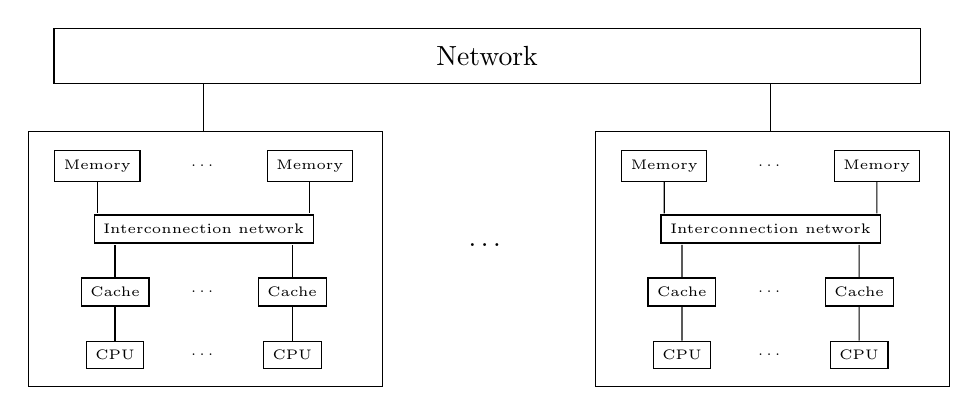
\begin{tikzpicture}[xscale = 0.45,yscale = 0.4]
\draw (11,3.5) node[draw, minimum height = 7mm, minimum width = 11cm]
  {Network};
%
\foreach \x in {0,16}{
  \draw(\x+0,0) node[place](mem1){\tiny Memory};
  \draw (\x+3,0) node{\tiny\ldots};
  \draw(\x+6,0) node[place](memn){\tiny Memory};
  %
  \draw(\x+3,-2) node[draw, minimum height = 2mm, minimum width = 2cm]
    {\tiny Interconnection network};
  \draw (mem1) -- ++ (0,-1.50); \draw (memn) -- ++ (0,-1.50); % Hack
  %
  \draw (\x+0.5, -4) node[place](cache1){\tiny Cache};
  \draw (\x+3,-4) node{\tiny\ldots};
  \draw (\x+5.5, -4) node[place](cachen){\tiny Cache};
  \draw (cache1) -- ++ (0,1.50); \draw (cachen) -- ++ (0,1.50);
  %
  \draw (\x+0.5,-6) node[place](cpu1){\tiny CPU};
  \draw (\x+3,-6) node{\tiny\ldots};
  \draw (\x+5.5, -6) node[place](cpun){\tiny CPU};
  \draw (cpu1) -- (cache1); \draw (cpun) -- (cachen);
  % Outer box and connection to network
  \draw (\x-1.95,1.1) -- ++ (10,0) -- ++ (0,-8.1) -- ++ (-10,0,0) -- cycle;
  \draw (\x+3,1.1) -- ++ (0,1.5);
}
\draw (11,-2.5) node{\ldots};
\end{tikzpicture}
\end{center}
\caption{A distributed-memory system composed of multiprocessor computers
  communicating over a network.}
\label{fig:distributed}
\end{figure}

%%%%%

Building a system like this is often more cost-effective than using a single
very large multiprocessor computer.  Such a system is easy to scale up, simply
by adding more computers.  Also, it can provide redundancy, being able to
continue even if one computer fails.  However, communication between
computers, over the network, is much slower than communication via shared
memory.

A \emph{grid system} is where a large number of computers work together.
These might be geographically distributed, and might belong to different
organisations.  The aim might be to share data, in a \emph{data grid}; or it
might be to share computational power, in a \emph{computational grid}; or it
might be to allow collaboration, in a \emph{collaborative grid}. 

\emph{Cloud computing} is essentially multicomputers for hire.  Individuals or
organisations can pay to use computing resources---either hardware or
software.  Whether this makes sense is mainly a financial decision.

%
%% \begin{center}
%% \ \includegraphics[width=6cm]{Pics/distributed.eps}\ 
%% \end{center}
% \framebox{Fig 1.3 from Andrews}
%
%%%%%

%% \begin{slide}
%% \heading{Distributed-memory multicomputers and networks}

%% A \emph{multicomputer} is a distributed-memory system where the processors are
%% physically close, connected by a high-speed interconnection network.

%% In \emph{network systems} (sometimes known as grids), processors
%% communicate over a network, such as a local area Ethernet or the
%% Internet.

%% One can, of course, build distributed-memory systems, where each computer is
%% itself a shared-memory multiprocessor.
%% % multicomputers from shared-memory multiprocessors.
%% \end{slide}

%% %%%%%

%% \begin{slide}
%% \heading{Grid systems and cloud computing}

%% Grid systems are large network systems, often sharing resources across
%% organisations.  They come in two main flavours:
%% %
%% \begin{description}
%% \item[Computational grids,] where computers work together on some
%%   computational task.
%%   % mostly used on problems that require little communication between the
%%   % subtasks. 

%% \item[Data grids,] where there is a huge amount of data to be processed.
%%   % Example types of data include the web (e.g.~web searching), astronomical
%%   % data, data from particle accelerators, genomic sequences.  The data grid may
%%   % be combined with a computational grid that operates on the data.
%% \end{description}


%% Cloud computing can be thought of as ``grids for hire''.  Companies ---such as
%% Amazon, HP, Google, Rackspace--- make grids of computers available to be hired
%% by organisations.  Whether to own your own grid or to hire is mainly an
%% economic decision. 
%% \end{slide}

%%%%%

%% \begin{slide}
%% \heading{Example: Google}

%% Google has 15 data centres worldwide, using about 900,000 servers.
%% %  between 500,000 and several
%% % million processors in total, grouped into clusters of a few thousand
%% % processors.\footnote{{\it Data-Intensive Supercomputing: The case for DISC},
%% %   Randal E. Bryant, CMU-CS-07-128.}
%% Each data centre stores several copies of the web (about 1.2 million terabytes)
%% % (about 200 terabytes),
%% together with indexes to allow efficient searching.  This is continually
%% updated by processes that crawl the web.

%% They use their own custom file system\footnote{{\it The Google File System}, 
%% Sanjay Ghemawat, Howard Gobioff, and Shun-Tak Leung,
%% \url{http://labs.google.com/papers/gfs.html}.}, to distribute the data across
%% servers, providing high performance and fault tolerance. 

%% Each web search uses about 1000 computers, in order to complete the search in
%% about 0.2 seconds.  

%% % Each web search requires about 10 seconds of computer time, but is completed
%% % in about 0.1 seconds by using multiple processors.

%% Their design uses hardware that is low-cost and low-power, rather than fast or
%% reliable. 

%% \vfill
%% \end{slide}
